\subsection{Ryan Rabinowitz}

I am currently enrolled in the Cybersecurity Master of Engineering program at the University of Colorado, Colorado Springs.
Some of my personal interests are 3D Printing (FDM only), Photography, Bowling, and flying my quadrocopter, I also have a small tabby cat named Morty. 
My research areas of interest are Computer Vision, Blockchain Systems, and Steganographic Systems, although I am interested in many projects involving cryptography that lie outside these topics. 

In CS 6000 I hope to start building on a wealth of skills required to create and publish meaningful research.
Namely, I would like to become more comfortable with LaTex and become more effective at skimming papers quickly. 
Co-authoring my first paper over the summer has gotten me familiar with overleaf and LaTex, but also revealed there is a long road ahead to mastery. 
As far as effective skimming of papers goes, I have read with care my entire life so skimming is somewhat counter-intuitive. 
From my understanding of CS 6000, I will be forced to confront this, which will be (hopefully) be a good thing.

A Git repo related to my research is RBF-Softmax \url{https://github.com/2han9x1a0release/RBF-Softmax.git}, a pytorch implementation of several common computer vision networks with Radial Basis Function-Softmax instead of a normal linear classifier head. 
The goal of RBF softmax is to shape the feature space of the network such that features of images within a given class are tightly clustered and class centers are spread apart from one another.
\begin{figure}[h]
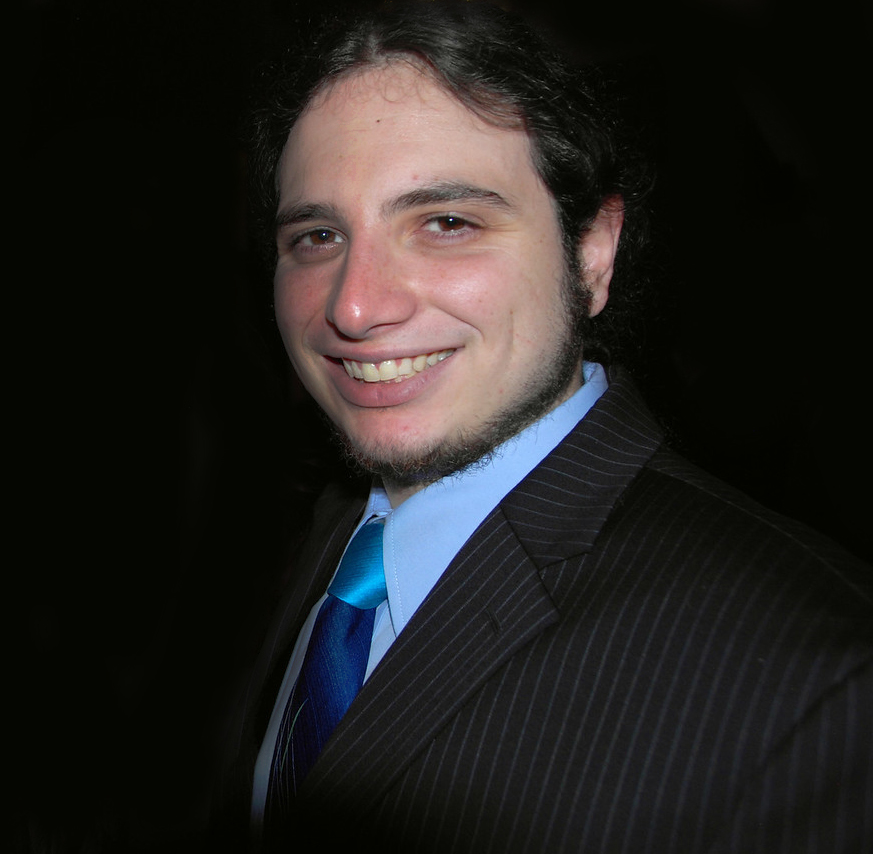
\includegraphics[width=8cm]{Rabinowitz_Headshot.jpg}
\end{figure}